\begin{tikzpicture}[scale=0.8,transform shape]
	\onslide<2->{ \node[] (input_taj) 
		{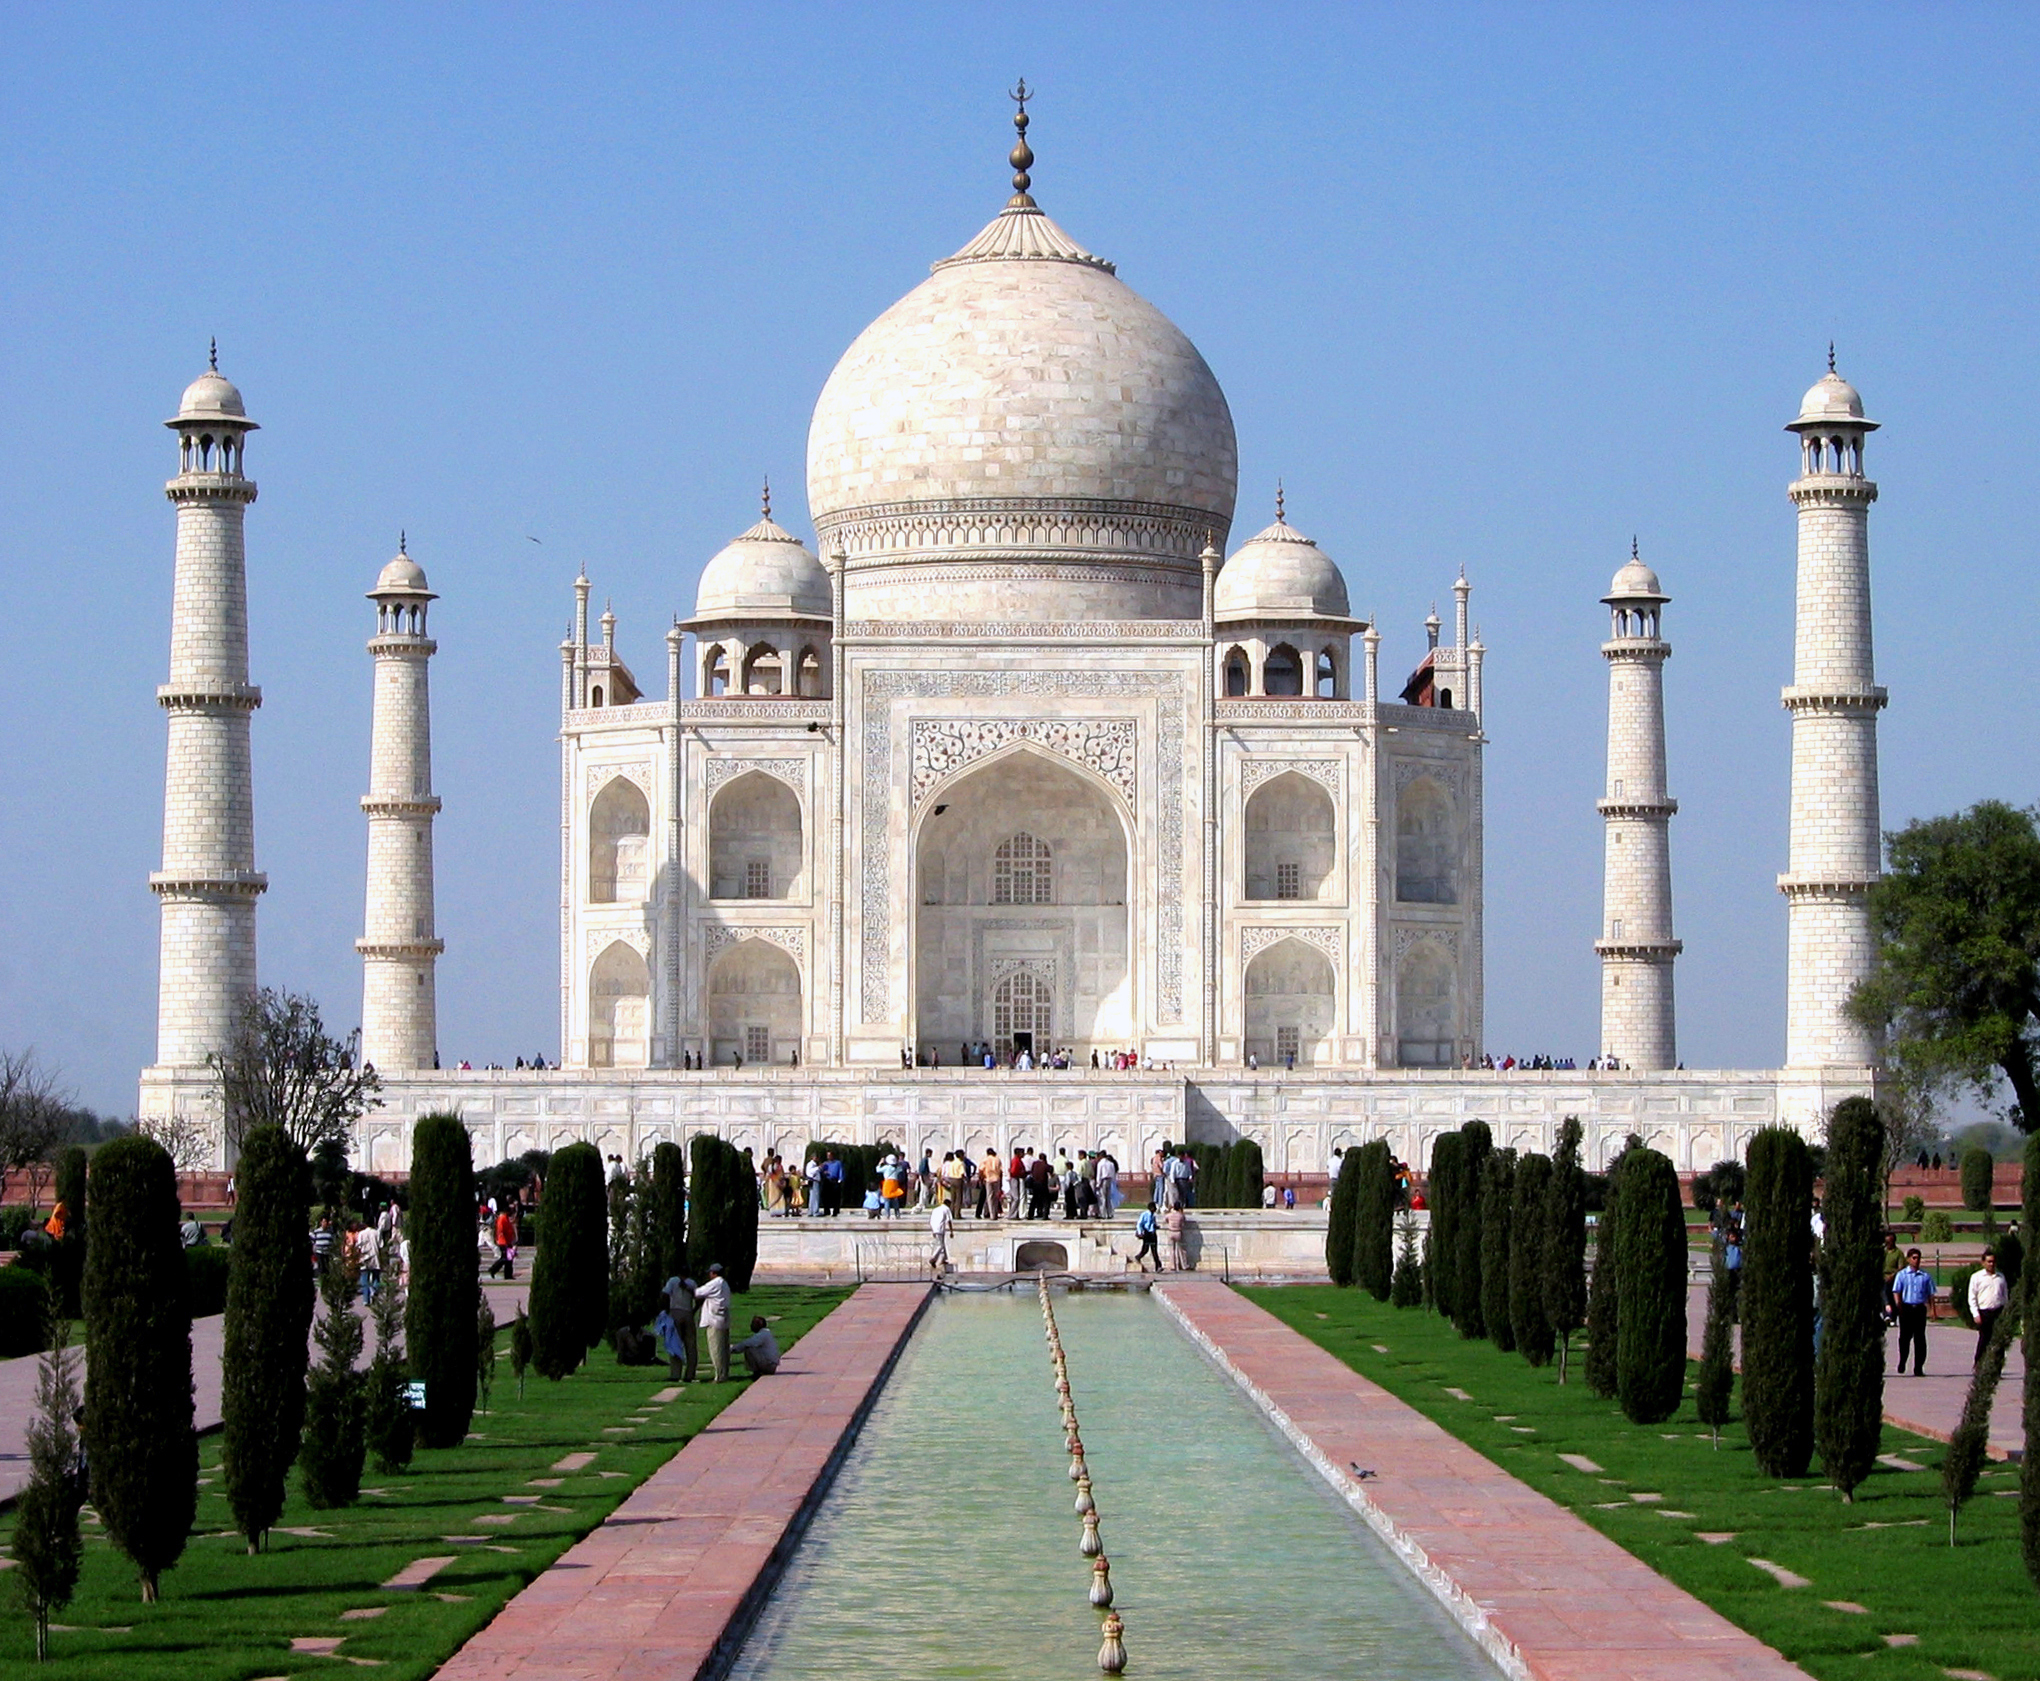
\includegraphics[width=20mm,height=17mm,scale=0.7]{images/taj_mahal.jpg}};}
	\onslide<2->{  
		\node  (raw1) at ($(input_taj) + (4.5,0)$) { 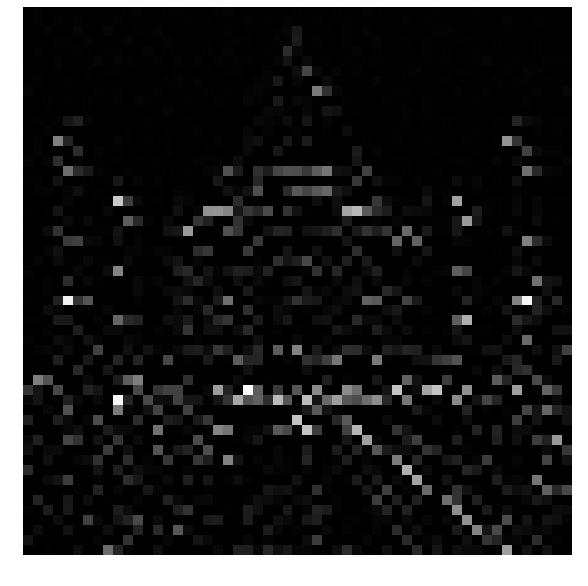
\includegraphics[width=20mm,height=17mm,scale=0.7]{images/convo1_2.png}};
		\node (raw2) at ($(raw1) + (-0.2,-0.2)$)  { 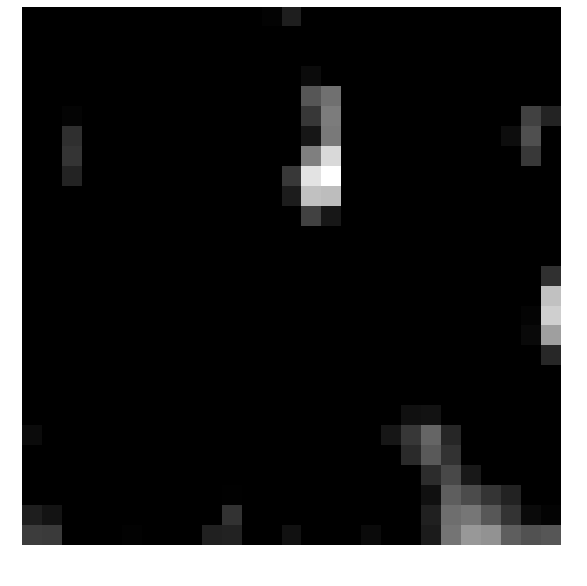
\includegraphics[width=20mm,height=17mm,scale=0.7]{images/convo2_2.png}};
		\node (raw3) at ($(raw2) + (-0.4,-0.2)$) { 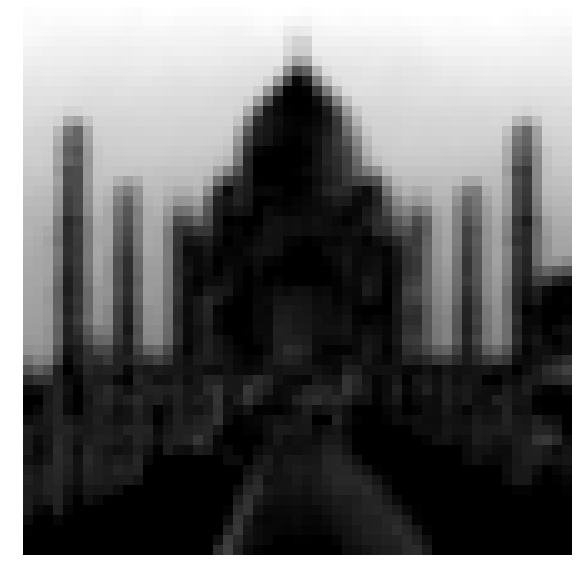
\includegraphics[width=20mm,height=17mm,scale=0.7]{images/convo1.png}};

		%\node[above of= raw,node distance=1.2cm ] (features)  {Features};
		\draw[->,thick] (input_taj) -- ($(raw1) + (-2,0)$) ;

	}
	\onslide<2->{

		\node (raw4) at ($(raw1) + (4.5,0)$)  { 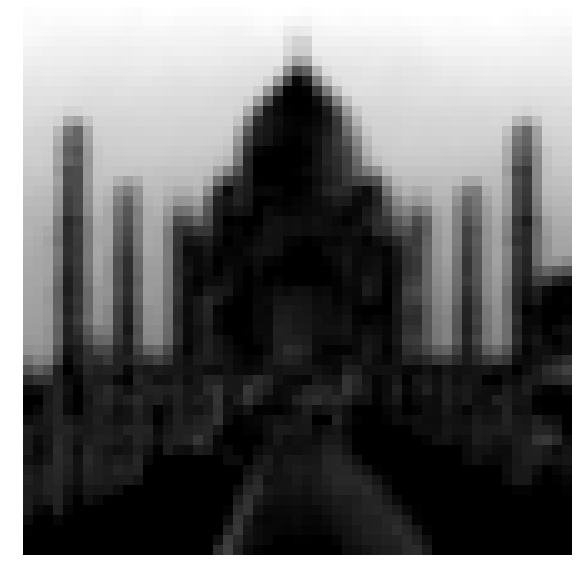
\includegraphics[width=20mm,height=17mm,scale=0.7]{images/convo1.png}};
		\node (raw5) at ($(raw4) + (-0.2,-0.2)$) { 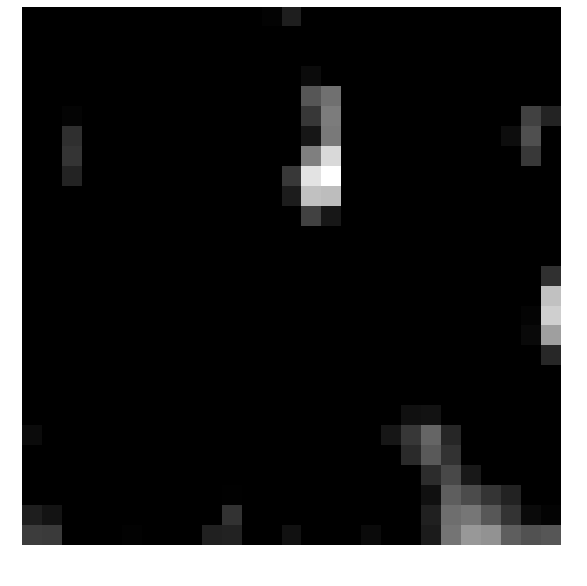
\includegraphics[width=20mm,height=17mm,scale=0.7]{images/convo2_2.png}};
		\node (raw6) at ($(raw5) + (-0.4,-0.2)$)  { 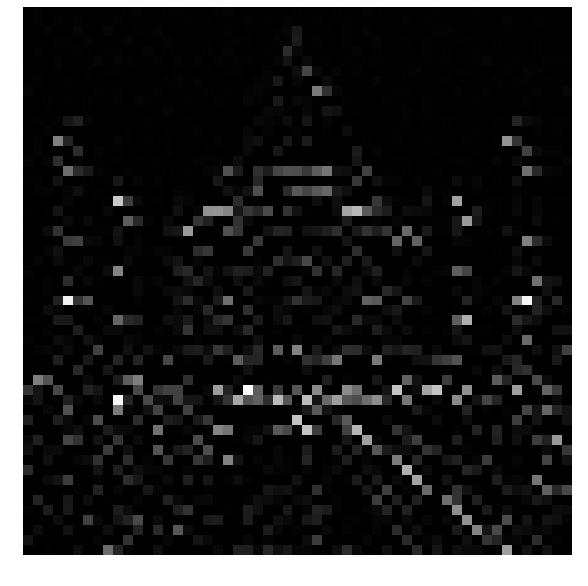
\includegraphics[width=20mm,height=17mm,scale=0.7]{images/convo1_2.png}};
		%\node[above of= raw,node distance=1.2cm ] (features)  {Features};

		\draw[->,thick] (raw1) -- ($(raw4) + (-2,0)$) ;
	}

	\onslide<2->{\node [right=4cm of raw4.center,anchor= center](output_taj){car, bus, \textcolor{blue}{monument}, flower};
		\draw[->,thick] (raw4) -- (output_taj) ;
		\node [] (o) at ($(output_taj) + (0,1.2)$) {\footnotesize{Classifier}};
		\node [] (i) at ($(input_taj) + (0,1.2)$) {\footnotesize{Input}};
	}


	\onslide<3->{\node [below of = output_taj,node distance=4.8em,anchor= center](back){\footnotesize{backpropagation}};
	}
	\onslide<3->{ 
		\node [below of = raw5,anchor=north] (edge2)  { \resizebox{25mm}{8mm}{ \begin{tabular}{ccccc}
			-0.01112582  & 0.02185669 & $\cdots$ & $\cdots$ & 0.00015161\\ 
			-0.00687587 & 0.01229961 & $\cdots$ & $\cdots$ & 0.00214013\\ 
			$\vdots$ & $\vdots$ &  &  & $\vdots$\\ 
			$\vdots$ & $\vdots$ &  &  & $\vdots$\\ 
			-0.00372989 & -0.00886137  &  $\cdots$ & $\cdots$ &-0.01974954 \\
			\end{tabular} }};
 
		\draw[->,thick] (back) -- ($(edge2) + (1.5,0.25)$) ;
	}
	\onslide<3->{
		\node [below of = raw2,anchor=north] (edge1)  { \resizebox{25mm}{8mm}{ \begin{tabular}{ccccc}
			-1.21358689e-03  & 3.23652686e-03 & $\cdots$ & $\cdots$ & -2.06615720e-02\\ 
			-1.52757822e-03  & 2.36130832e-03 & $\cdots$ & $\cdots$ & -1.19824838e-02\\ 
			$\vdots$ & $\vdots$ &  &  & $\vdots$\\ 
			$\vdots$ & $\vdots$ &  &  & $\vdots$\\ 
			-8.25322699e-04 & -5.14897937e-03 &  $\cdots$ & $\cdots$ &-9.90395527e-03 \\
			\end{tabular} }};
		\draw[->,thick] (edge2) -- (edge1) ;   
	}


\end{tikzpicture}